\section{Simulator implementation details}

\subsection{Simulator Structure}
In order to roll a die in the simulator, Bullet requires user to render a world before putting in the object. We then create a rigid body object with some initial conditions, step the simulation by some amount of time in the Simulator and check if the velocity of the object has dropped to zero in all x,y,z directions, then check its ending orientation to see which face has it landed on.\\\\
The first problem we encountered is that Bullet does not automatically calculate center of mass (com) and moment of inertia (moi) for convex hull shape objects. We used Mirtich algorithm to calculate com and moi for arbitrary convex shape objects. (details)\\\\
The second problem we have is debugging. Unlike most programs, where the programmer knows the desired output of the execution, here we cannot easily correct ourselves by just looking at the probabilities produced by the simulator. We used several methods to help our debugging.\\
\begin{itemize}
    \item Base line object. Although we do not know what probabilities a particular configuration of the cuboid die can produce, we do know for a cube-shaped die, all faces should have equal probability, so if the outcome deviates from those numbers, we know something is wrong with our code.\\
    \item Simulation invariants. For the same configuration, the simulator should produce similar results over large number of runs. If there is a significant bias towards certain sides or does not produce repeatable results over same configurations, we know something is wrong with our code.\\
    \item GUI outputs. The simulator do provide a visual output for a single roll, so we can manually inspect if the generated die looks correct. For example, the way we found out the com calculation is wrong is by holding one side of the die stable in the GUI and see if it can reach a stable state. The default settings put com at (0,0,0) so when we held the die on that vertex it keeps spanning even when no other force is applied to it.\\
    \item Theoretical result. In one paper (citation needed) the authors found one set of theoretical probabilities for rolling a cuboid die on a smooth surface with side length 13,20,23 centimeters. Though the conditions might not be exactly the same, it provides some reference as how the simulation results should be for that particular configuration.
    
\end{itemize}

\subsection{Unbiased rolling}
One of the greatest advantages of the simulator comparing to the real life rolling is that we can guarantee from a theoretical standpoint that the rolling direction is uniformly sampled from all possible directions. We decided to use Quaternions to denote our initial rotation, since the alternative method, Euler angles, is not easy to sample evenly over all possible configurations. \\\\
The sample space for initial orientation of the die can be denoted as a certain degree of rotation along a particular axis. We can denote all possible directions as a sphere's surface, and therefore we should sample uniformly from within a sphere with 2${pi}$ radius. At first we were only doing three uniform samples for x,y,z to get the axis, and that leads to sampling biased towards one vertex of the box.\\\\
\begin{figure}[h]
\center
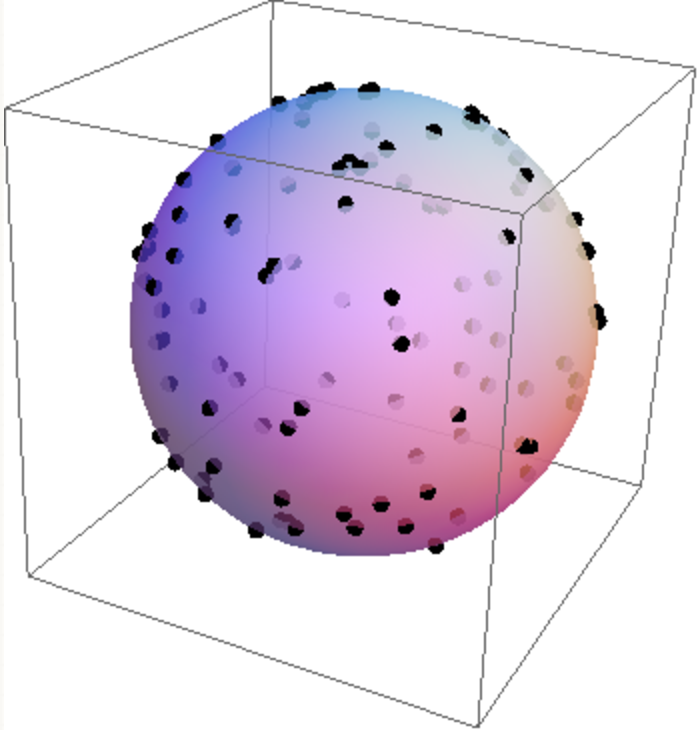
\includegraphics[scale=0.5]{sphereInAbox.png}
\caption{Sampling from a box versus a sphere (citation needed)}
\label{fig:square_p}
\end{figure}\\\\
The other choice we face is with the initial speed and angular velocity. Although it's easier to sample uniformly from all possible configurations, we have a problem with scale. What maximum speed should we pick? Making the die with higher initial energy might lead to different results. Although we do not have a theoretical justification for under what maximum speed should the die produce random results, we do know the maximum speed and height of the rolling should not exceed what normal students can achieve in a limited experiment. So we used the techniques mentioned above to see what speeds produced the desired outcome of the die and adjusted accordingly. In the end we picked our maximum speed to be 10m/s and our maximum angular velocity to be 10${pi}$/s.

\subsection{Simulator accuracy}
The simulator can produce reasonable results for simple objects. However for the purpose of this project our requirement for accuracy might be greater than what the simulator could sustain. For example the optimal discrepancy for a six-sided die is below 1\%, which means the result generated by the simulator needs to be within 1\% of the true distribution.\\\\
This may or may not be achievable by the simulator for a couple reasons. One of them is that we as programmers are not very familiar with underlying physics of the simulator structure. During one experiment we rolled a cuboid die along x axis with no initial speed or angular velocity, which means it should never land on two of the sides. The simulator produced the expected result with very small probabilities on those two sides, which implies it might added on some additional physics conditions that we might be unaware of, like air friction.\\\\
Another example to demonstrate this is with the scale of the object. When our input is larger than 1 meters for the cuboid, the edges between vertexes mostly resemble lines. However when the size gets smaller, the edges become thicker and may become a side themselves. This phenomenon might be caused by the fact that Bullet is using tetrahedron to generated convex hull shape objects, and its accuracy decreases when the size of the object is too small. These problems could significantly increase the errors generated in the simulation.
\begin{figure}[h]
\center
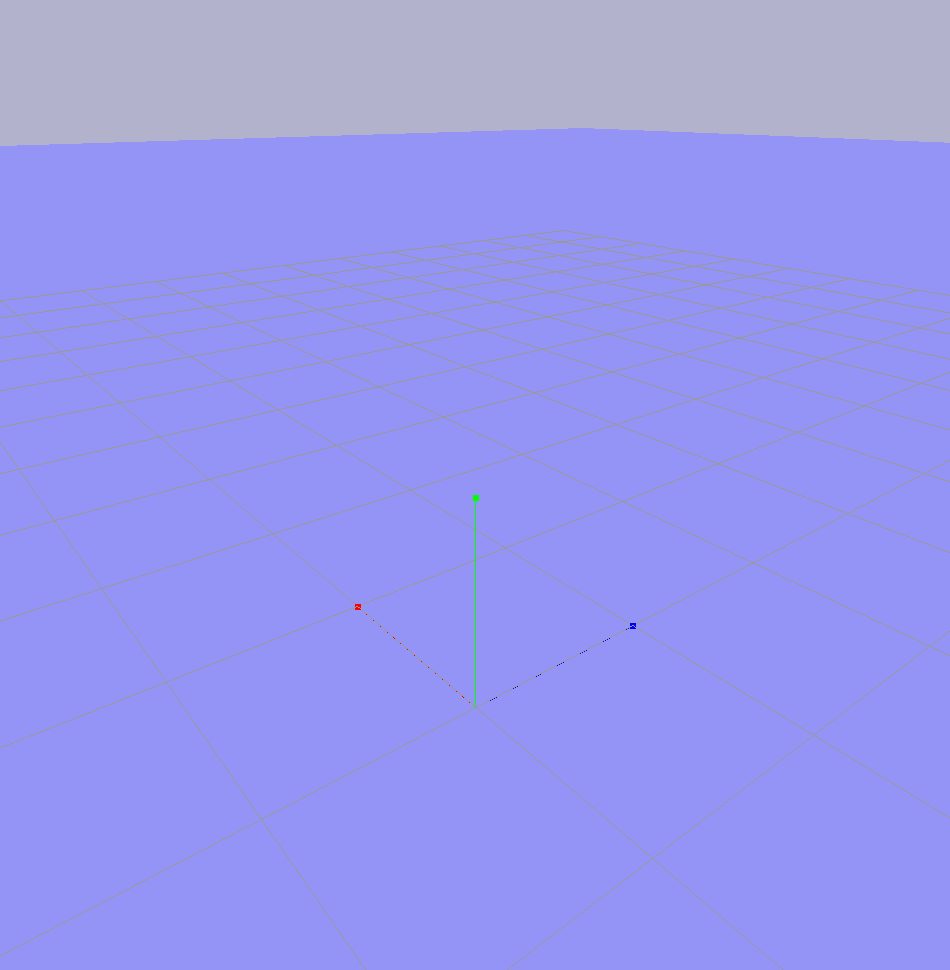
\includegraphics[scale=0.8]{bullet_axis.png}
\caption{axises in bullet; the x,y,z axis is denoted by red, green, blue; therefore rotation against x axis cannot create above zero probabilities for two out of six sides for a cuboid die.}
\label{fig:square_p}
\end{figure}
\begin{figure}[h]
\center
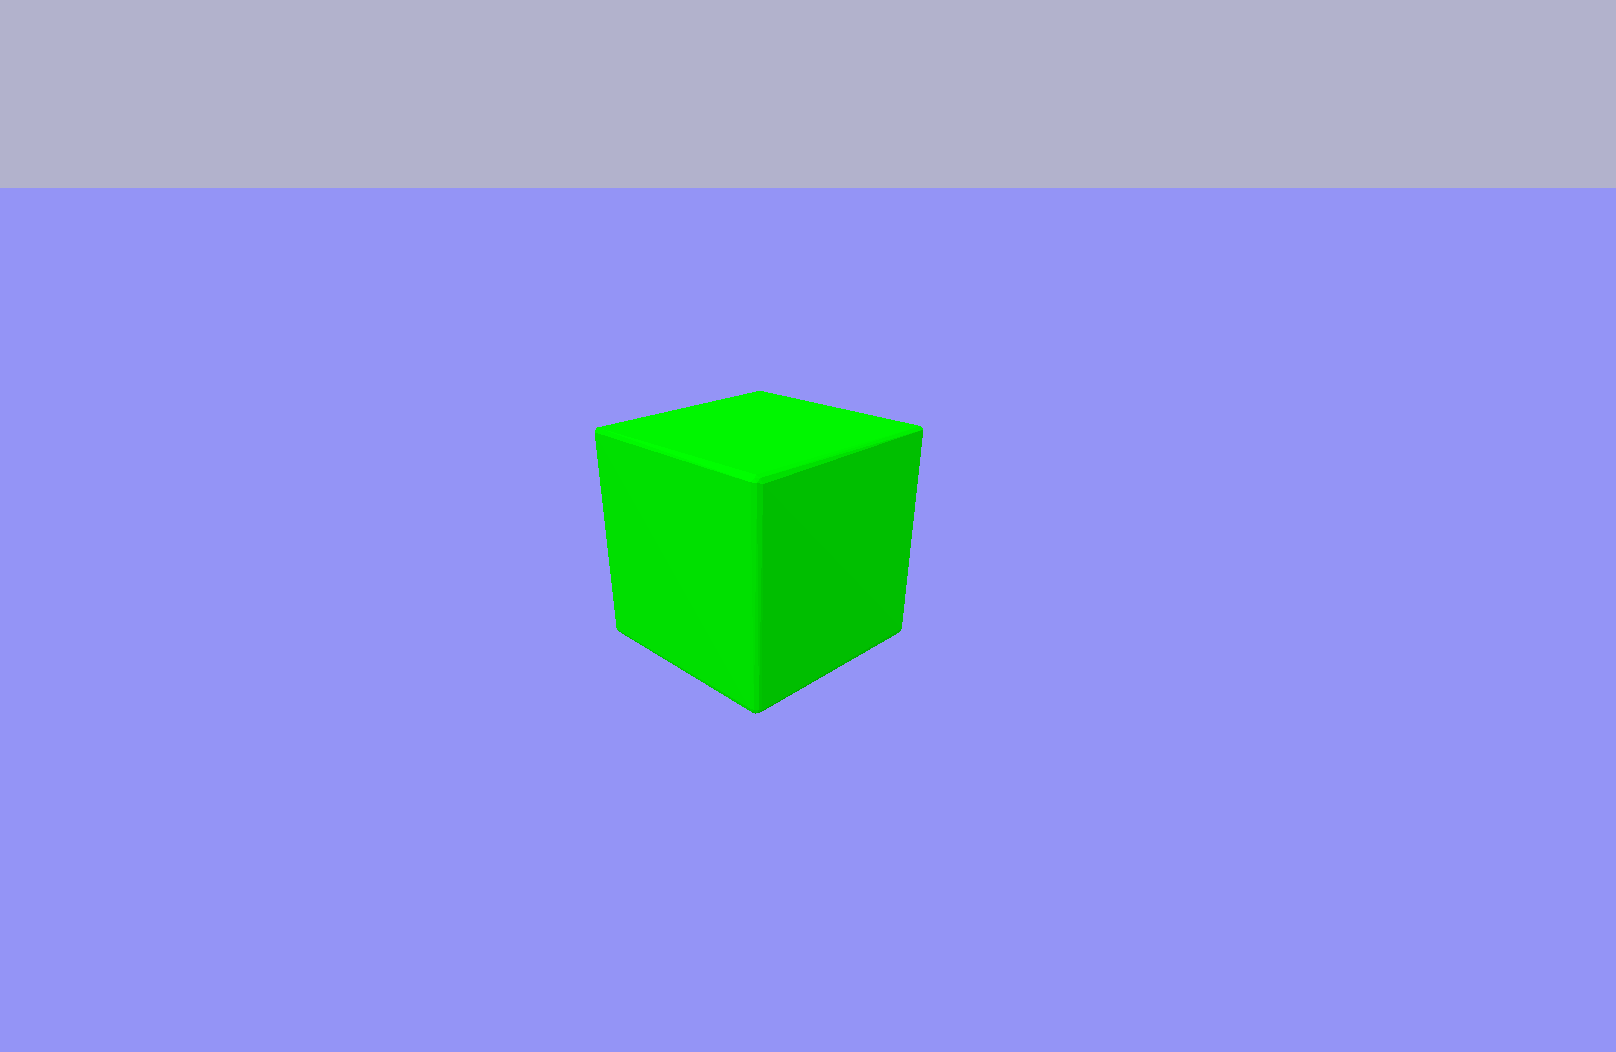
\includegraphics[scale=0.5]{normal_cuboid.png}
\caption{A 1m side length cube in bullet; most of the edges look straight.}
\label{fig:square_p}
\end{figure}\\\\
\begin{figure}[h]
\center
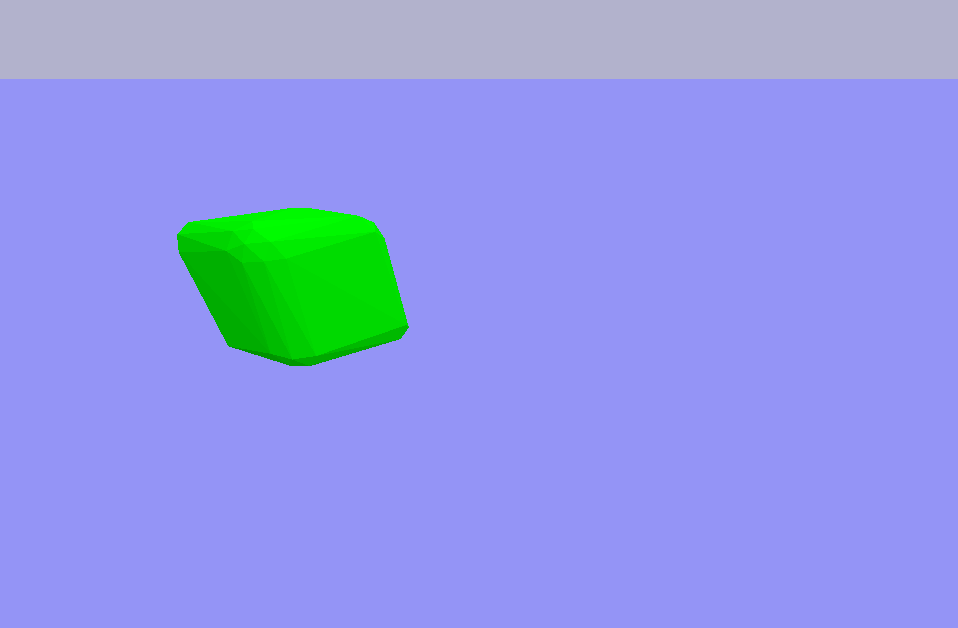
\includegraphics[scale=0.8]{small_cuboid.png}
\caption{A 0.1m side length cube in Bullet; one can see its edges are resembling faces rather than a line.}
\label{fig:square_p}
\end{figure}\\\\